%!TEX root = lec07_documents.tex

\newsavebox\bibliographyOne
\begin{lrbox}{\bibliographyOne}
\begin{lstlisting}[style=markup]
<bibliography>
  <book>
    <title>The Book of Why</title>
    <author>Perl</author>
    <author>Mackenzie</author>
    <publisher>Basic Books</publisher>
    <year>2018</year>
  </book>
  <book>
    <title>The Art of Computer Programming</title>
    <author>
      <first>Donald</first>
      <last>Knuth</last>
    </author>
    <published>Addison-Wesley, 1969</published>
  </book>
</bibliography>
\end{lstlisting}
\end{lrbox}

\begin{frame}
Example XML document for the next few slides:

\begin{center}
\begin{tikzpicture}[every node/.style={inner sep=0,outer sep=0}]
\node<+-> at (0,0) [anchor=south west] {\scalebox{0.75}{\usebox{\bibliographyOne}}};

\begin{scope}[on background layer]
\onslide<2|handouts:1>{
  \fill [orange!10] (0.35,1) rectangle (3.5,2.35);
  \draw [->,red,thick] plot [smooth] coordinates {(0.35, 1.8) (-0.5,2.2) (-0.5, 4) (0.35, 4.4)};
  \node [red, anchor=east] at (-0.65,2.75) {($\dagger$)};
}
\onslide<3|handouts:1>{
  \fill [blue!10] (0.35,0.65) rectangle (6,0.975);
  \draw [->,blue,thick] plot [smooth] coordinates {(6, 0.8) (6.5,1.2) (6.5, 3) (5, 3.4)};
  \node [blue, anchor=west] at (6.75,2) {($\ddagger$)};
}
\end{scope}
\end{tikzpicture}
\end{center}

\uncover<+->{
\begin{itemize}[noitemsep]
\onslide<2-3|handouts:1>{\item[\textcolor{red}{($\dagger$)}] Elements need not have the same kind of content!}
\onslide<3|handouts:1>{\item[\textcolor{blue}{($\ddagger$)}] Missing or new elements are also possible.}
\end{itemize}}

\end{frame}

\begin{frame}{Data Model}

XML elements (including the entire document) are modeled as \textbf{ordered labeled trees}.

\begin{center}
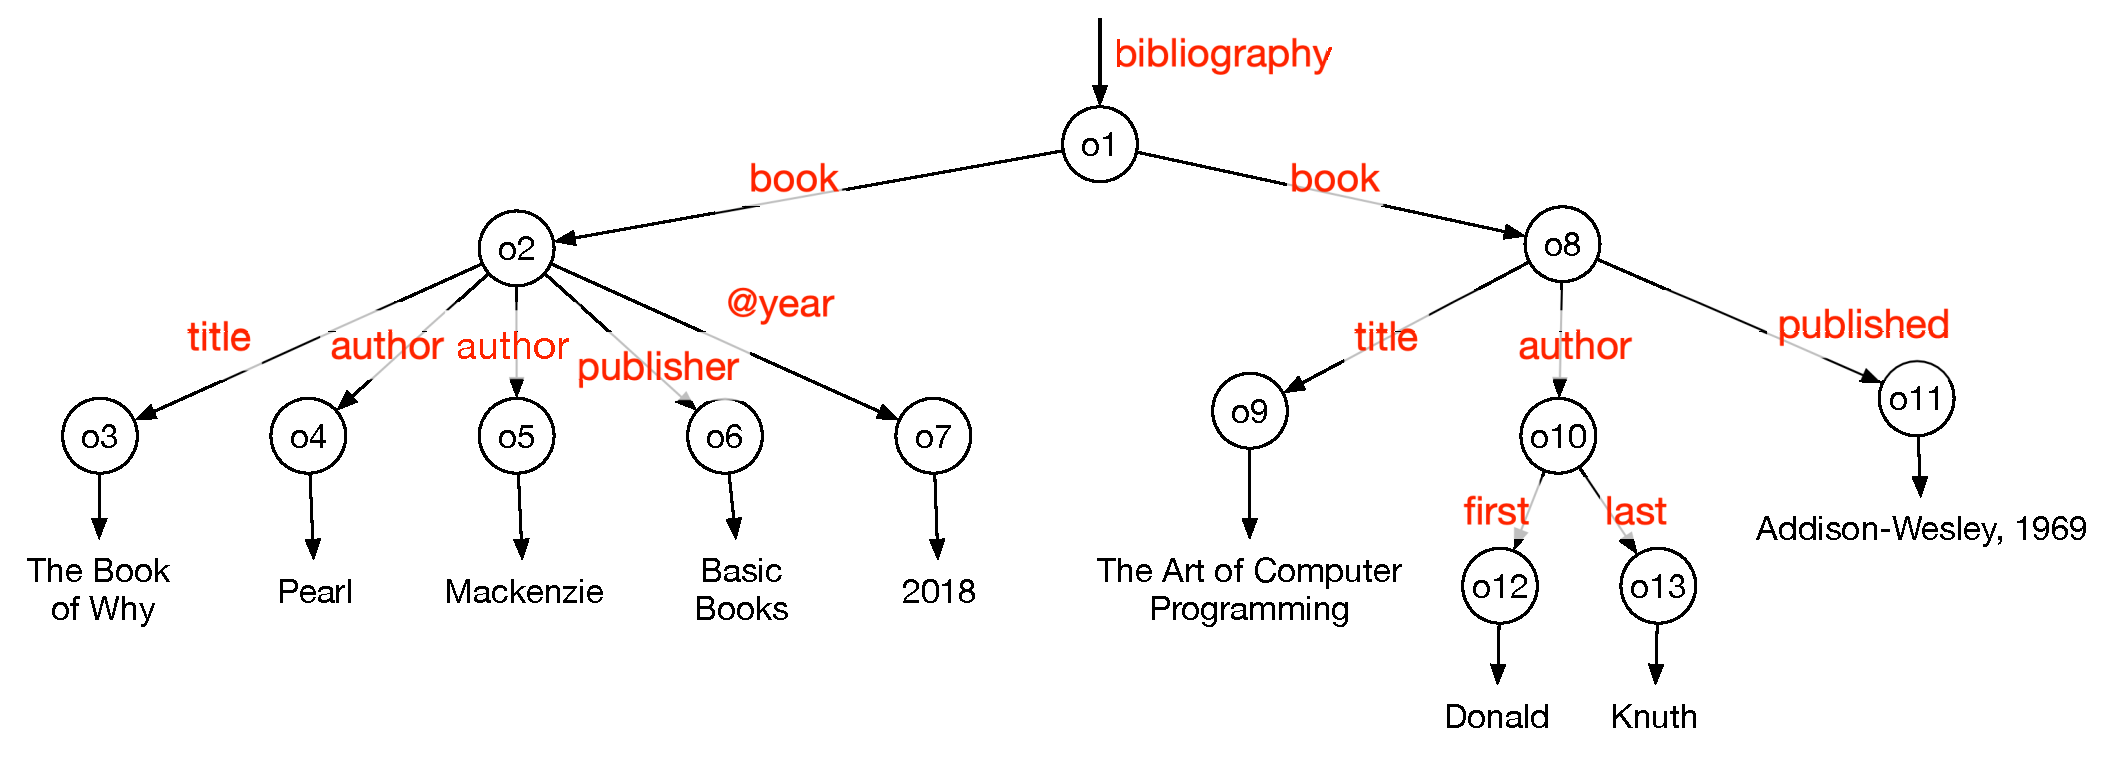
\includegraphics[width=\textwidth]{figures/XML_data_model.eps}
\end{center}

\vskip1em

XML is a \textbf{semi-structured} data format: different elements with the same label can have different types or different kinds of content.

\end{frame}

\begin{frame}{XML Query Languages}

The W3C defines (at least) two query languages for XML, which are used \textbf{together}. 

\begin{BOX}{XPath}
\begin{itemize}[-,noitemsep]
\item like regular expressions, but on paths over XML trees
\item specifies and ``returns'' nodes in the tree
\end{itemize}
\end{BOX}

\begin{BOX}{XQuery}
\begin{itemize}[-,noitemsep]
\item functional query language that computes an answer from input XML documents
\item uses XPath to locate nodes in the input (like the \lstinline{WHERE} clause in SQL) that are used to compute the answer
\end{itemize}
\end{BOX}

\end{frame}

\begin{frame}[fragile]{XPath}

XPath is a language for \textbf{addressing} parts of an XML document, designed to be used by both XSLT and XPointer. (\url{https://www.w3.org/TR/1999/REC-xpath-19991116/})

\begin{itemize}[-,topsep=-5pt,noitemsep]
\item Contains approximately 200 built-in functions.
\item A major element in the XML ecosystem, including XSLT, XLink, and XQuery.
\end{itemize}

\vskip1em

\lstset{language=XPath}

Every XPath expression returns \textbf{\alert{an ordered sequence}} of nodes in the XML tree. 

Unless otherwise specified, the ordering of the nodes is the \emph{document ordering}.

\end{frame}


\begin{frame}{XPath}

An XPath expression is a called a \alert{location \textbf{path}}:

\begin{block}{\alert{Location Path}}
A location path is a \textbf{sequence} of \blue{location \textbf{steps}}, separated by \alert{/}, that identifies one or more nodes in a \textbf{document}.
\end{block}

\vskip1em

\textbf{Example:} \fbox{\lstinline[style=XQuery]!doc("books.xml")/child::bibliography/child::book!}

\vskip1em

Each \textbf{Location \blue{Step}}:
\begin{itemize}[-,noitemsep,nolistsep,topsep=-0.5em]
\item Specifies a single navigational step in a path;
\item Is evaluated against a single \alert{context node}, and returns a \alert{\textbf{sequence} of nodes};
\item Almost always consists of a \alert{navigational axis} and a \alert{node test}.
\end{itemize}


\end{frame}

\begin{frame}[fragile]{Location Steps}

\textbf{Formally}: \fbox{\lstinline[style=XQuery]{axis::node test-:[:-predicate-:]:-}}
\begin{itemize}[-,noitemsep,topsep=-0.5em]
\item \textbf{Node tests} are optional. Often they are \alert{name tests} (i.e., an element or attribute name).

\item \textbf{Predicates} are also optional, and are used to filter nodes reachable using the axis and satisfying the name test.

\end{itemize}

\vskip1em

Most \textbf{common axes} and their \textbf{abbreviated forms}:
\begin{center}
\begin{tabular}{c|c|l}
axis & abbreviation & example\\
\hline
child & \lstinline[style=XQuery]!-:/:-! & \lstinline[style=XQuery]!doc("books.xml")-:/:-bibliography! \\
descendant-or-self & \lstinline[style=XQuery]!-://:-! & \lstinline[style=XQuery]!doc("books.xml")-://:-book! \\
attribute & \lstinline[style=XQuery]!-:@:-! & \lstinline[style=XQuery]!//book/-:@:-year! \\
self & \lstinline[style=XQuery]!-:.:-! & \lstinline[style=XQuery]!//author[-:.:-/last = 'Knuth']! \\
ancestor & \lstinline[style=XQuery]!-:..:-! & \lstinline[style=XQuery]!//first[-:..:-/last = 'Knuth']!
\end{tabular}
\end{center}


\end{frame}

\begin{frame}[fragile]

\lstset{language=XPath}

\hspace*{-2em}
\begin{tikzpicture}
\node at (0,0) [anchor=south west] {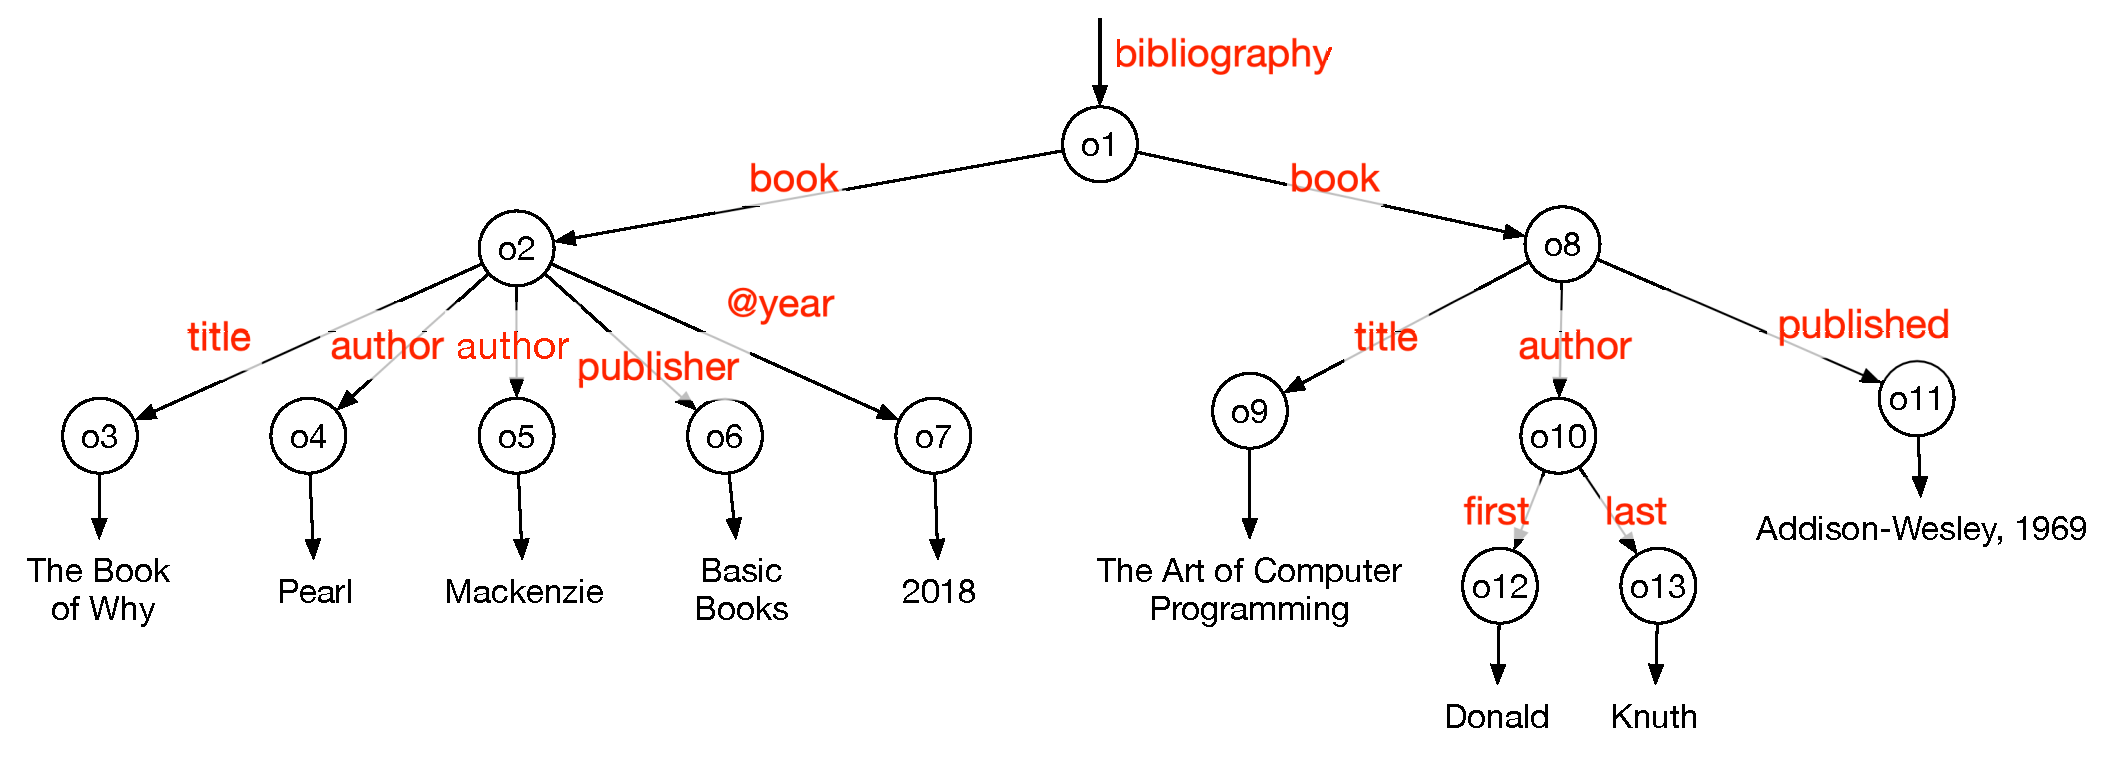
\includegraphics[width=1.1\textwidth]{figures/XML_data_model.eps}};

\node (p1) at (0,-1) [anchor=west] {\lstinline[style=Xquery]{/bibliography/book/@year}  = };
\node (p2) at (0,-2) [anchor=west] {\lstinline[style=Xquery]{/bibliography//author}  =  };
\node (p3) at (0,-3) [anchor=west] {\lstinline[style=Xquery]{//first/../author}  = };
\onslide<2-| handout:1>{\node [blue,yshift=2pt,right= 0.25cm of p1] {( o7 )};}
\onslide<3-| handout:1>{\node [blue,yshift=2pt,right= 0.25cm of p2] {( o4, o5, o10 )};}
\onslide<4-| handout:1>{\node [blue,yshift=2pt,right= 0.25cm of p3] {( o10 )};}
\end{tikzpicture}
\end{frame}


\newsavebox\personXML
\begin{lrbox}{\personXML}
\begin{lstlisting}[style=markup]
<?xml version="1.0"?>
<people>
  <person born="1912" died="1954">
    <name>
      <first>Alan</first>
      <last>Turing</last>
    </name>
    <profession>computer scientist</profession>
    <profession>mathematician</profession>
    <profession>cryptographer</profession>
  </person>
  <person born="1918" died="1988">
    <name>
      <first>Richard</first>
      <middle_initial>P</middle_initial>
      <last>Feynman</last>
    </name>
    <profession>physicist</profession>
    <hobby>Playing the bongoes</hobby>
  </person>
</people>
\end{lstlisting}
\end{lrbox}


\begin{frame}{Comparison Expressions}

XPath and XQuery model XML have multiple comparators.

\begin{center}
\begin{tabular}{c|c|c}
\blue{General} & \alert{Value} & \\
\blue{Comparator} & \alert{Comparator} & \raisebox{0.5em}{Description} \\
\hline
\lstinline[style=XQuery]{-:=:-} & \lstinline[style=XQuery]{eq} & Equals\\
\lstinline[style=XQuery]{-:!=:-} & \lstinline[style=XQuery]{ne} & Not equals\\
\lstinline[style=XQuery]{-:>:-} & \lstinline[style=XQuery]{gt} & Greater than \\
\lstinline[style=XQuery]{-:>=:-} & \lstinline[style=XQuery]{ge} & Greater than or equals to\\
\lstinline[style=XQuery]{-:<:-} & \lstinline[style=XQuery]{lt} & Less than\\
\lstinline[style=XQuery]{-:<=:-} & \lstinline[style=XQuery]{le} & Less than or equals to
\end{tabular}
\end{center}

\vskip1em

\blue{General} comparators can be used to compare \blue{values and sequences}, while \alert{value} comparators can \alert{only} be used to compare two \alert{values}.

\end{frame}


\begin{frame}[fragile]

\hspace*{-2em}
\begin{tikzpicture}
\node at (0,0) [anchor=south west] {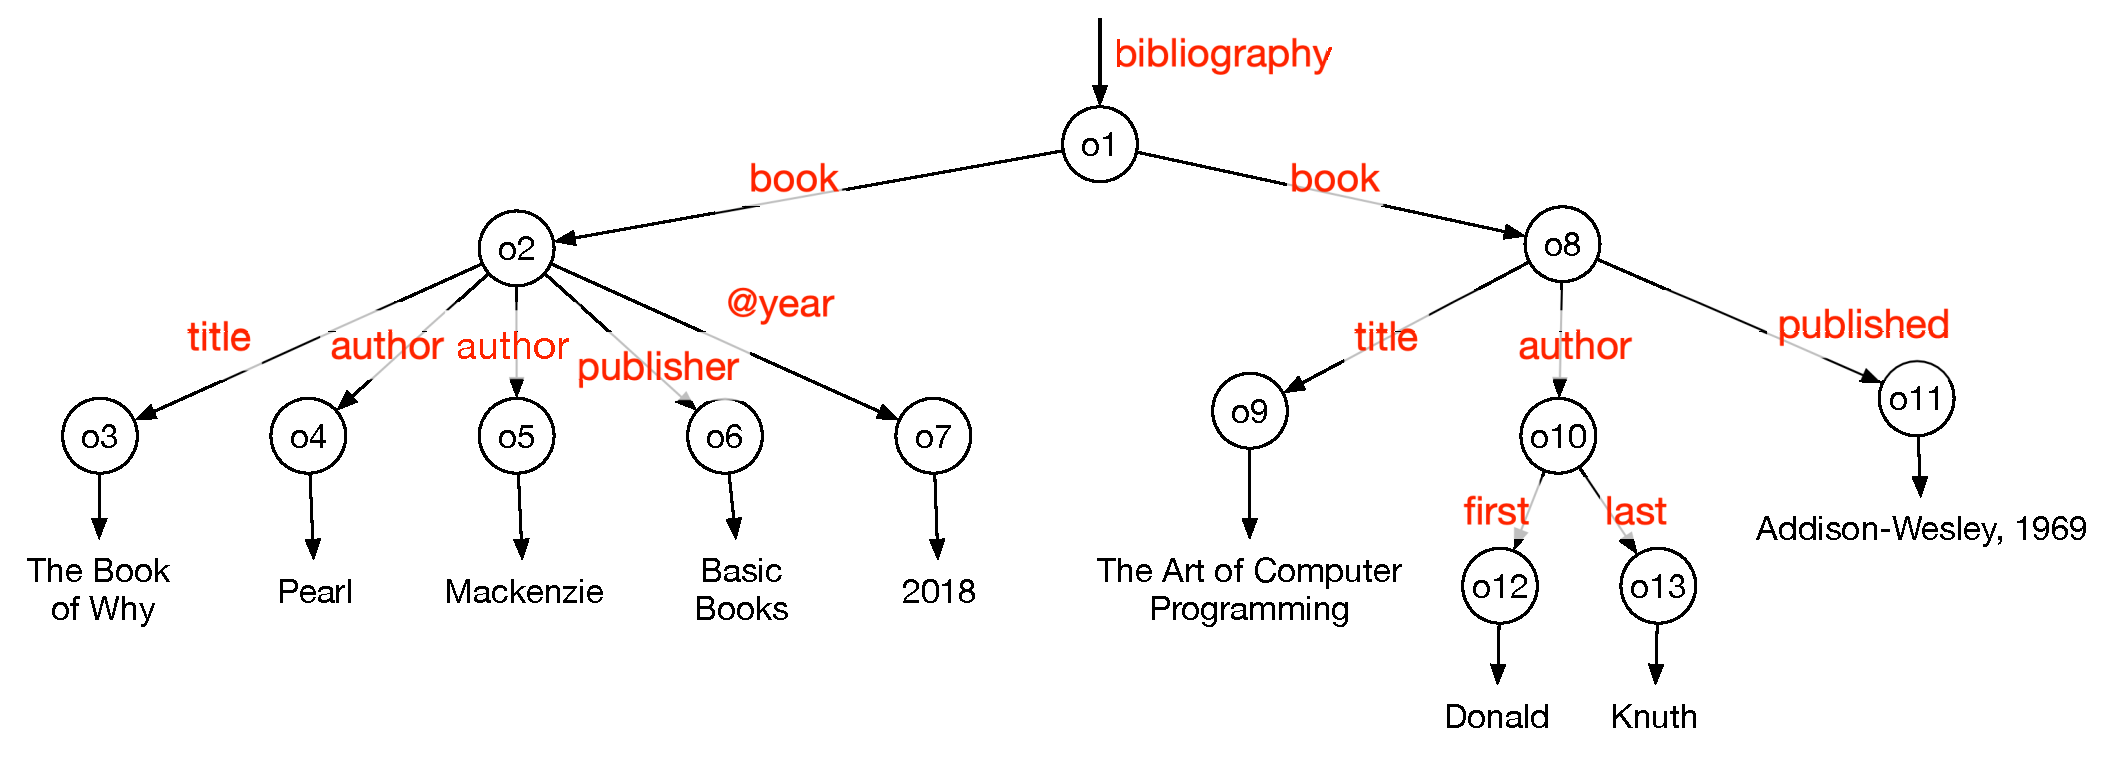
\includegraphics[width=1.1\textwidth]{figures/XML_data_model.eps}};
\end{tikzpicture}

\textbf{Example}: selecting books  written by \lstinline[style=XQuery]{Pearl}... because there can be many (i.e., a sequence) of authors in each book, we need to use the general comparator:

\begin{center}
\fbox{\lstinline[style=XQuery]{//book[./author -:=:- 'Pearl']}}
\end{center}

The comparison above evaluates to true if \emph{at least one} item in the sequence is equal to the value \lstinline[style=XQuery]{Pearl}.

\end{frame}


\begin{frame}[fragile]

Why do we need value comparators? 

Why not just use general comparators?

\vskip1em

\begin{block}{Defensive programming}
Comparisons involving sequences can lead to confusing results. If you \emph{know} that the comparison should involve a single value (e.g., every book has only one isbn) it is best to use a value comparator.
\end{block}

\vskip1em

With defensive programming, if you get an error, at least you know that the document is not structured as you expected.


\end{frame}



\begin{frame}[fragile]{More XPath}

\vskip1em

\lstset{style=cmput391,language=XPath}

\begin{columns}[onlytextwidth]
\begin{column}{0.5\textwidth}

\textbf{Wildcards}: \alert{\lstinline[style=XQuery]!//person/-:@*:-!}
\begin{itemize}[-,topsep=-0.5em]
\item Returns all attributes of any person.
\end{itemize}

\vskip1em

\textbf{Disjunctions}: \alert{\lstinline[style=XQuery]!//-:(:-first-:|:-last-:):-!}
\begin{itemize}[-,topsep=-0.5em]
\item Returns all elements named \lstinline[style=XQuery]!first! or \lstinline[style=XQuery]!last!.
\end{itemize}

\vskip1em

\textbf{Filters}: \alert{\lstinline[style=XQuery]!//person-:[:-./profession="physicist"-:]:-!}
\begin{itemize}[-,topsep=-0.5em]
\item Returns \lstinline{person} elements that contain a child called \lstinline[style=XQuery]{profession} whose value is the string \lstinline[style=XQuery]{"physicist"}.
\end{itemize}

\end{column}
\begin{column}{0.5\textwidth}
\vskip1em
\scalebox{0.8}{\usebox\personXML}
\end{column}
\end{columns}
\end{frame}



\begin{frame}[fragile]{Variables in Predicates are Existentially Quantified}

\vskip2em

\lstset{language=XPath}

\textbf{Logical test} \alert{\lstinline!//person[./profession="mathematician"]!} returns \lstinline{person} elements that contain \textbf{at least one child} called \lstinline{profession} whose value is the string \lstinline{"mathematician"}.

 \vskip2em

 \begin{lstlisting}[style=markup]
 <person born="1912" died="1954">
    <name>
      <first>Alan</first>
      <last>Turing</last>
    </name>
    <profession>computer scientist</profession>
    <profession>mathematician</profession>
    <profession>cryptographer</profession>
</person>
 \end{lstlisting}

\end{frame}

\begin{frame}{Functions}

XPath 2.0 and XQuery 1.0 share the same function library\footnote{\url{https://www.w3.org/TR/xpath-functions-31/}}
\begin{itemize}[-,noitemsep,topsep=-0.5em]
\item Became a recommendation in Jan 2007.
\item With approximately 200 functions.
\item More were added over time.
\end{itemize}
 

\vskip1em

Every function is evaluated with respect to a context node
  the higher-level specification in which XPath is used, such as XSLT or XPointer, decides how this context node is determined

\vskip1em

XPath is weakly typed
  automatic type conversions (casting) are done whenever possible

\end{frame}


\begin{frame}[fragile]

XPath defines a ``Core Function Library'' that every implementation \textbf{must} provide:

\begin{itemize}[-,topsep=-5pt]
\item \alert{Node Set Functions} operate on properties of XML nodes\\
~~\textbf{ex:} \XPath{id("046509760X")/author[position()=1]} selects the first \lstinline!author! child of the element whose \lstinline[language=DTD]!-:#ID:-! attribute equals 046509760X.

\item \alert{String Functions}: usual string manipulation found in most programming languages (sub-strings, concatenation, etc.)

\item \alert{Boolean Functions}: \XPath!and()!, \XPath!or()!, \XPath!not()! plus \XPath!boolean(X)! which converts object X into a boolean, returning:\\
~~-~ \textbf{True} if X is one of: a positive number, a non-empty string, or a non-empty node set.\\
~~-~ \textbf{False} otherwise.
\end{itemize}

\end{frame}


\begin{frame}[fragile]

XPath ``Core Function Library'' continued:

\begin{itemize}[-]

\item \alert{Number Functions} manipulate numbers and cast strings as numbers.
\begin{itemize}[-,noitemsep,topsep=-5pt]
\item \XPath!number(X)! converts strings spelling numeric values (e.g., \lstinline!"123.45"!) into proper numbers
\item \XPath!number(X)! converts booleans into numbers (true:1, false:0)
\item \XPath!sum()! returns the sum of a sequence of numbers
\item \XPath!floor()!, \XPath!ceiling()! and \XPath!round()! work as defined in most programming languages
\end{itemize}
\end{itemize}

\vskip1em
\begin{BOX}{Programming Languages and XML}
Unlike with SQL, the W3C approach with XPath/XQuery was to provide \textbf{many functions} programmers would be familiar with.
\end{BOX}

\end{frame}


\begin{frame}[fragile]{XQuery -- FLOWR Expressions}

Main clauses in XQuery since version 1.0:

% \lstset{style=cmput391,language=XPath}

\begin{center}
\begin{minipage}{0.5\textwidth}
\begin{lstlisting}[style=XQuery]
[for -|variable bindings|-]
[let -|variable bindings|-]
[where -|condition(s)|-]
[order by -|criteria|-]
[return -|expression|-]
\end{lstlisting}
\end{minipage}
\end{center}

\vskip2em

\begin{itemize}[-,noitemsep]
\item \lstinline[style=Xquery]!for! clause: create tuple streams
\item \lstinline[style=Xquery]!let! clause: bind variables to results of expressions
\item \lstinline[style=Xquery]!where! clause: filter tuples that don’t satisfy a condition
\item \lstinline[style=Xquery]!order by! clause: sort the tuples in the tuple stream
\item \lstinline[style=Xquery]!return! clause: builds the result of the expression for each tuple in the stream 
\end{itemize}
\end{frame}


\newsavebox\FROMbox
\begin{lrbox}{\FROMbox}
\lstinline[language=SQL]!FROM!
\end{lrbox}
\newsavebox\SELECTbox
\begin{lrbox}{\SELECTbox}
\lstinline[language=SQL]!SELECT!
\end{lrbox}
\newsavebox\WHEREbox
\begin{lrbox}{\WHEREbox}
\lstinline[language=SQL]!WHERE!
\end{lrbox}

\newsavebox\forBOX
\begin{lrbox}{\forBOX}
\lstinline[style=XQuery]!for!
\end{lrbox}
\newsavebox\whereBOX
\begin{lrbox}{\whereBOX}
\lstinline[style=XQuery]!where!
\end{lrbox}
\newsavebox\returnBOX
\begin{lrbox}{\returnBOX}
\lstinline[style=XQuery]!return!
\end{lrbox}



\begin{frame}[fragile]{XQuery -- analogy to SQL}

Like with SQL and relational data, most XML queries perform three major tasks:

\begin{enumerate}[(1)]
\item Specify a \alert{scope} (i.e., identify data elements are relevant to the query)
\item Specify \alert{filters} to remove undesirable elements
\item \alert{Compute} a result from the elements that remain
\end{enumerate}

\vskip1em

\begin{columns}[onlytextwidth]
\begin{column}{0.4\textwidth}
Equivalence between SQL and XQuery clauses.
\end{column}
\begin{column}{0.5\textwidth}
\begin{tabular}{c|c|c}
\textbf{task} & SQL & XQuery\\
\hline\hline
(1) & \usebox{\FROMbox} & \usebox{\forBOX}\\
(2) & \usebox{\WHEREbox} & \usebox{\whereBOX}\\
(3) & \usebox{\SELECTbox} & \usebox{\returnBOX}
\end{tabular}
\end{column}
\end{columns}
\end{frame}



\newsavebox\biblioXML
\begin{lrbox}{\biblioXML}
\begin{lstlisting}[style=markup]
<books>
  <book year="2009">
    <title>Causality</title>
    <author><last>Pearl</last><first>Judea</first></author>
    <publisher>Cambridge</publisher>
  </book>
  <book year="1999">
    <title>Foundations of Statistical Natural Language Processing</title>
    <author><last>Manning</last><first>Christopher</first></author>
    <author><last>Schütze</last><first>Hinrich</first></author>
    <publisher>MIT Press</publisher>
  </book>
  <book year="2005">
    <title>Introduction to Information Retrieval</title>
    <author><last>Manning</last><first>Christopher</first></author>
    <author><last>Raghavan</last><first>Prabhakar</first></author>
    <author><last>Schütze</last><first>Hinrich</first></author>
    <publisher>Cambridge</publisher>
  </book>
</books>
\end{lstlisting}
\end{lrbox}


\begin{frame}[fragile]{Example document -- books.xml}
\vspace*{-0.5em}\scalebox{0.85}{\usebox\biblioXML}
\end{frame}



\begin{frame}[fragile]{XQuery expressions}

Prototypical simple XQuery query:

\vskip1em

\begin{columns}[onlytextwidth]
\begin{column}{0.5\textwidth}
\begin{lstlisting}[style=XQuery]
for $b in doc("books.xml")//book
where $b/@year eq "2009"
return $b/title
\end{lstlisting}
\end{column}

\begin{column}{0.4\textwidth}
\begin{onlyenv}<2-| handouts:1>
\begin{lstlisting}[style=markup]
<title>Causality</title>
\end{lstlisting}
\end{onlyenv}
\end{column}

\end{columns}


\vskip1em

Evaluation algorithm

\begin{enumerate}[(a),topsep=-5pt]
\item Compute path expression \lstinline[language=XPath]!doc("books.xml")//book!
\item For each element \lstinline[style=XQuery]!$b! in the result, if \lstinline[style=XQuery]!$b! satisfies the \lstinline[style=XQuery]!where! clause, evaluate the \lstinline[style=XQuery]!return! clause, \emph{appending} to the final result.
\end{enumerate}

\end{frame}

\begin{frame}[fragile]{The \lstinline[style=XQuery]!return! Clause}

Like with SQL, an XQuery query can compute \alert{new} values. 

For example, we can create new XML elements that were not in the document

\vskip1em

\begin{columns}[onlytextwidth]
\begin{column}{0.5\textwidth}
\begin{lstlisting}[style=XQuery]
for $b in doc("books.xml")//book
where $b/@year eq "2009"
return <newElement> 
  { $b/title/text() }
</newElement>
\end{lstlisting}
\end{column}

\begin{column}{0.45\textwidth}
\begin{onlyenv}<2-| handouts:1>
\begin{lstlisting}[style=markup]
<newElement>Causality</newElement>
\end{lstlisting}
\end{onlyenv}
\end{column}
\end{columns}

In XQuery, we compute the values that go inside elements (or attributes) with expressions within brackets: \lstinline[style=cmput391]!-:{:- ... -:}:-!

\end{frame}

\begin{frame}[fragile]{Using the \lstinline[style=XQuery]!let! Clause as ``CTEs''}
\vskip1em
\begin{lstlisting}[style=XQuery]
let $CUPauthors := for $b in doc("books.xml")//book
                   where $b/publisher eq "Cambridge"
                   return $b/author
for $a in $CUPauthors
return <author>{ $a/first/text() , " " , $a/last/text()}</author>
\end{lstlisting}

\vskip1em

in XQuery, commas are used for concatenating the values of expressions:

\begin{onlyenv}<2-| handouts:1>
\begin{lstlisting}[style=markup]
<author>Judea Pearl</author>
<author>Christopher Manning</author>
<author>Prabhakar Raghavan</author>
<author>Hinrich Schütze</author>
\end{lstlisting}
\end{onlyenv}
\end{frame}

\begin{frame}[fragile]{Sequences}

XQuery is a functional language; its basic abstraction is \alert{iterating over \textbf{ordered} sequences} of data elements.

\vskip1em

\begin{itemize}[-]
\item The \lstinline[style=XQuery]!let! clause \textbf{binds} sequences to variables.
\begin{lstlisting}[style=XQuery]
let $books := doc("books.xml")//book
\end{lstlisting}
Think of \lstinline[style=XQuery]!$books! as an array or linked list with the book elements.

\item The \lstinline[style=XQuery]!for! clause \textbf{binds} items in a sequence to a variable.
\begin{lstlisting}[style=XQuery]
let $books := doc("books.xml")//book
for $b in $books
\end{lstlisting}

\begin{block}{Document Ordering!}
\alert{Unless otherwise specified}, the order of the items in the sequence is \alert{the same} as in the document.
\end{block}

\end{itemize}
\end{frame}

\begin{frame}[fragile]{Positional Predicates}

Because sequences are ordered, we can use positional predicates to filter out items.

The following query returns the title of the second book in the document:

\begin{lstlisting}[style=XQuery]
for $b in doc("books.xml")//book[position() = 2]
return $b/title
\end{lstlisting}
\vspace*{-1em}
The test above can be abbreviated as \lstinline[style=XQuery]!doc(...)//book[-:2:-]!.

\vskip1em
The following returns the last author of every book.

\begin{lstlisting}[style=XQuery]
for $b in doc("books.xml")//book
return $b/author[position() = count($b/author)]
\end{lstlisting}
\vspace*{-1em}
The test above can be abbreviated as \lstinline[style=XQuery]!$b/author[last()]!.

\end{frame}


\begin{frame}[fragile]{Operations on Sequences}
See: \url{https://www.w3.org/TR/xpath-functions-31/#sequence-functions}

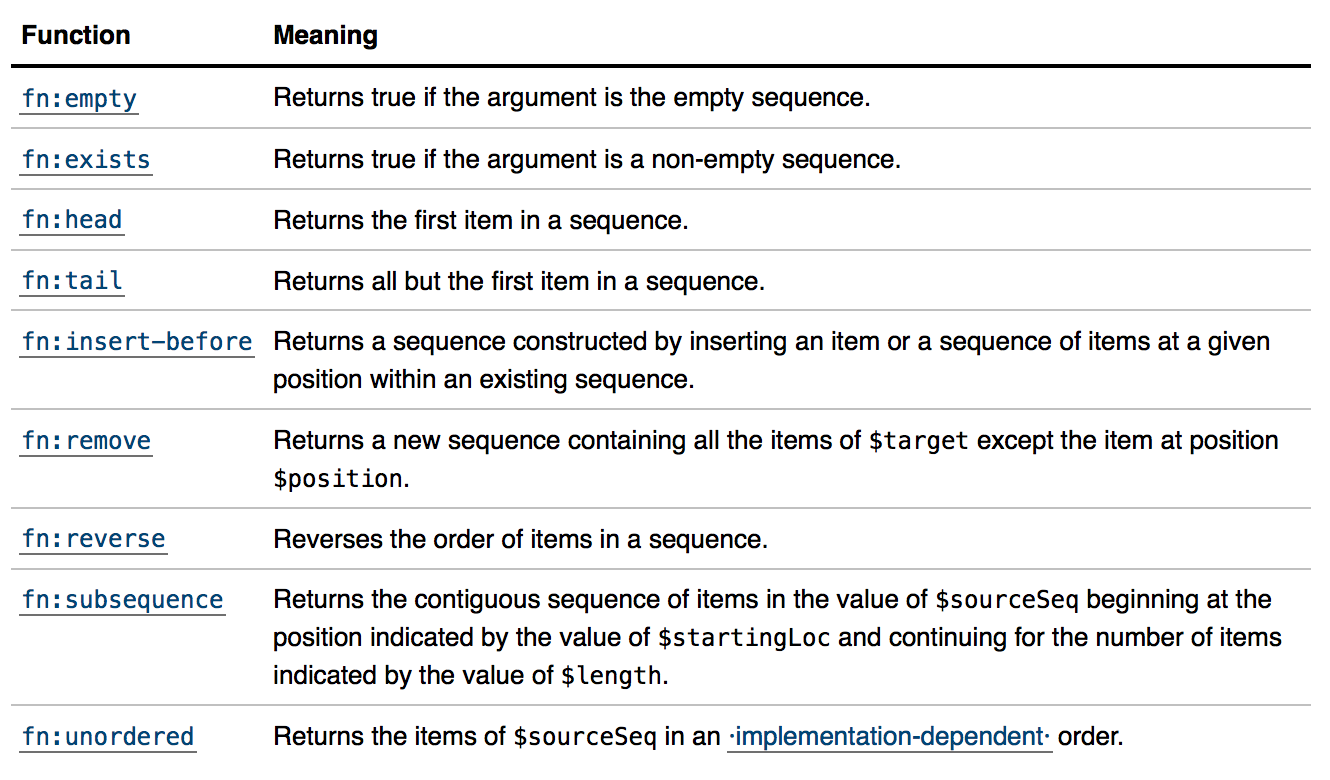
\includegraphics[width=\textwidth]{figures/XQuery_sequence_functions1.png}

\end{frame}

\begin{frame}[fragile]
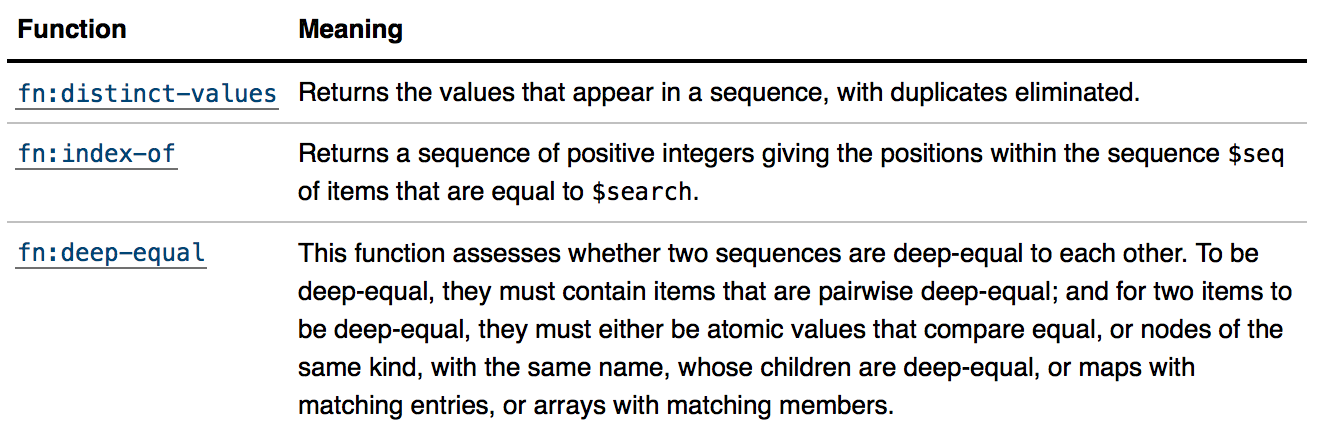
\includegraphics[width=\textwidth]{figures/XQuery_sequence_functions2.png}

Example:

\begin{lstlisting}[style=XQuery]
for -:$n:- in distinct-values(doc("books.xml")//publisher/text())
return <publisher>{-:$n:-}</publisher>
\end{lstlisting}

\begin{onlyenv}<2-| handouts:1>
\begin{lstlisting}[style=markup]
<publisher>Cambridge</publisher><publisher>MIT Press</publisher>
\end{lstlisting}

\vskip1em

Why do we \textbf{need} \lstinline[style=XQuery]!text()! in the path expression above?
\end{onlyenv}
\end{frame}


\begin{frame}[fragile]
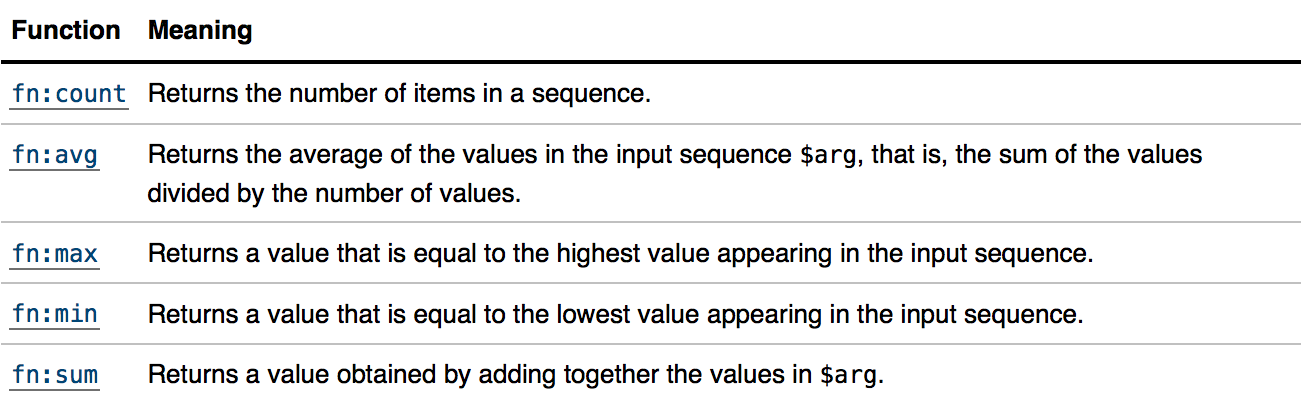
\includegraphics[width=\textwidth]{figures/XQuery_sequence_functions3.png}

Example:

\begin{lstlisting}[style=XQuery]
let -:$cnts:- := for $b in doc("books.xml")//book
             return count($b/author)
return round(avg(-:$cnts:-), 2)
\end{lstlisting}

\begin{onlyenv}<2-| handouts:1>
\begin{lstlisting}[style=markup]
2
\end{lstlisting}
\end{onlyenv}
\end{frame}

\begin{frame}[fragile]{Comparisons Involving Sequences}

Recall the \alert{general comparators} that apply to values and sequences:

\begin{itemize}[noitemsep]
\item \lstinline[style=XQuery]!-:=:-! (equals to) \qquad\qquad\qquad \lstinline[style=XQuery]{-:!=:-} (different than)
\item \lstinline[style=XQuery]!-:<:-! (less than) \qquad\qquad\qquad \lstinline[style=XQuery]!-:<=:-! (less than or equal to)
\item \lstinline[style=XQuery]!-:>:-! (greater than) \qquad\qquad~~ \lstinline[style=XQuery]!-:>=:-! (greater than or equal to)
\end{itemize}

\vskip1em

\begin{block}{Existential Semantics}
\lstinline[style=XQuery]!$s1  OP $s2! evaluates to \textbf{true} if \underline{there exist} items \alert{\texttt{x}} in \lstinline[style=XQuery]!$s1! and \alert{\texttt{y}} in \lstinline[style=XQuery]!$s2! for which \lstinline[style=XQuery]!x OP y! is true.
\end{block}

Examples: all programs below return \textbf{true}...

\begin{columns}[onlytextwidth]
\begin{column}{0.3\textwidth}
\begin{lstlisting}[style=XQuery]
let $s1 := (1,2,3)
let $s2 := (1,2)
return $s1 = $s2
\end{lstlisting}
\end{column}

\begin{column}{0.3\textwidth}
\begin{lstlisting}[style=XQuery]
let $s1 := (1,2,3)
let $s2 := (1,2)
return $s1 @< $s2
\end{lstlisting}
\end{column}

\begin{column}{0.3\textwidth}
\begin{lstlisting}[style=XQuery]
let $s1 := (1,2,3)
let $s2 := (1,2)
return $s1 > $s2
\end{lstlisting}
\end{column}
\end{columns}
\end{frame}


\begin{frame}[fragile]
\textbf{\blue{Comparisons with sequences can be convenient...}}

\vskip0.5em

\textbf{Ex:} find the titles of books that have at least one author whose first name is Prabhakar

\begin{lstlisting}[style=XQuery]
for $b in doc("books.xml")//book
where $b/author/first/text() = "Prabhakar"
return $b/title
\end{lstlisting}

Returns

\begin{lstlisting}[style=XQuery]
<title>Introduction to Information Retrieval</title>
\end{lstlisting}

\vskip1em

Why? For that book, we have that \\ \lstinline[style=XQuery]!$b/author/first/text()! $\leftarrow$ \lstinline[style=XQuery]!("Christopher", "Prabhakar", "Hinrich")!.

\end{frame}


\begin{frame}[fragile]

XQuery uses \alert{casting} aggressively, in an attempt to simplify the queries. The following expression from the previous query compares two \textbf{sequences}:

\begin{center}
\lstinline[style=XQuery]!$b/author/first/text() = "Prabhakar"!
\end{center}

% \vskip1em

XQuery casts the RHS to \lstinline[style=XQuery]!( "Prabhakar" )!

The following query (note it does not have \lstinline[style=XQuery]!text()!) computes the same answer:

\begin{lstlisting}[style=XQuery]
for $b in doc("books.xml")//book
where $b/author/first = "Prabhakar"
return $b/title
\end{lstlisting}

XQuery understands the RHS is a sequence of values, and casts each \lstinline[style=XQuery]!<first>! element into the corresponding value.

\end{frame}


\begin{frame}[fragile]
\textbf{\blue{But comparisons with sequences can also be confusing...}}

\textbf{Ex:} find the titles of books that have at least one author whose first name is Prabhakar and last name is Manning. 

\begin{lstlisting}[style=XQuery]
for $b in doc("books.xml")//book
where $b/author/first = "Prabhakar" and $b/author/last = "Manning"
return $b/title
\end{lstlisting}

The query ``should return nothing'' (as there is no author satisfying the conditions). Yet, it returns:

\begin{lstlisting}[style=XQuery]
<title>Introduction to Information Retrieval</title>
\end{lstlisting}

\vskip1em

Why? For that book, both \\\lstinline[style=XQuery]!("Christopher", "Prabhakar", "Hinrich") = "Prabhakar"! and \\ \lstinline[style=XQuery]!("Manning", "Raghavan", "Schütze") = "Manning"! evaluate to true.

\end{frame}


\begin{frame}[fragile]
Fixing the query so that it finds correctly the titles of books that have at least \emph{one author} whose first name is Prabhakar and last name is Manning.

\begin{lstlisting}[style=XQuery]
for $b in doc("books.xml")//book
where $b/author/first = "Prabhakar" and $b/author/last = "Manning"
return $b/title
\end{lstlisting}

\vskip1em 

\begin{onlyenv}<2-| handouts:1>
\begin{lstlisting}[style=XQuery]
for $b in doc("books.xml")//book
  for $a in $b/author
  where $a/first = "Prabhakar" and $a/last = "Manning"
  return $b/title

\end{lstlisting}
\end{onlyenv}

\end{frame}



\begin{frame}[fragile]{Nested Loops}

\begin{columns}[onlytextwidth]
\begin{column}{0.4\textwidth}

The previous query is an example of a \emph{correlated} nested loop:

\vskip2em

\begin{lstlisting}[style=XQuery]
for $b in doc("books.xml")//book
   for $a in $b/author
      return $a/last
\end{lstlisting}

\vskip1em

\begin{onlyenv}<2-| handouts:1>
\begin{lstlisting}[style=markup]
<last>Pearl</last>
<last>Manning</last>
<last>Schütze</last>
<last>Manning</last>
<last>Raghavan</last>
<last>Schütze</last>
\end{lstlisting}
\end{onlyenv}
\end{column}

\begin{column}{0.5\textwidth}
\scalebox{0.75}{\clipbox{0pt -1pt 3em 0.5em}{\scalebox{0.75}{\usebox\biblioXML}}}
\end{column}

\end{columns}
\end{frame}

\begin{frame}[fragile]{Products and Joins}

We write cross products explicitly as nested loops:

\begin{columns}
\begin{column}{0.5\textwidth}
\begin{lstlisting}[style=XQuery]
let $s1 := (1,2,3)
let $s2 := (1,2)
for $a in $s1
  for $b in $s2
  return <pair>{ $a , ":" , $b }</pair>
\end{lstlisting}
\end{column}
\begin{column}{0.25\textwidth}
\begin{lstlisting}[style=XQuery]
<pair>1 : 1</pair>
<pair>1 : 2</pair>
<pair>2 : 1</pair>
<pair>2 : 2</pair>
<pair>3 : 1</pair>
<pair>3 : 2</pair>
\end{lstlisting}
\end{column}
\end{columns}

\vskip1em

Recall a join is a cross product followed by a selection...

\begin{columns}
\begin{column}{0.5\textwidth}
\begin{lstlisting}[style=XQuery]
let $s1 := (1,2,3)
let $s2 := (1,2)
for $a in $s1
  for $b in $s2
  where $a eq $b
  return <pair>{ $a , ":" , $b }</pair>
\end{lstlisting}
\end{column}
\begin{column}{0.25\textwidth}
\begin{lstlisting}[style=XQuery]
<pair>1 : 1</pair>
<pair>2 : 2</pair>
\end{lstlisting}
\end{column}
\end{columns}
\end{frame}

\begin{frame}[fragile]{More Joins}

Suppose we have two XML files: \lstinline!books.xml! as before and \lstinline!loans.xml! to keep track of books loaned out to library users.

The following query joins the two files, returning the titles of the books which are loaned and due (at the date the query executes).

\vskip1em

\begin{lstlisting}[style=XQuery]
let $due := for $h in doc("holdings.xml")//loan
  where $h/due eq current-date()
  return $h
for $b in doc("books.xml")//book
   for $h in $due
   where $h/@isbn eq $b/@isbn
   return $b/title
\end{lstlisting}

\end{frame}


\begin{frame}[fragile]{Aggregation in XQuery 1.0}

XQuery V1.0 does not have an explicit clause for aggregation, unlike SQL. Aggregation can still be accomplished through nested loops.

\textbf{Example:} counting the books per publisher.

\begin{lstlisting}[style=XQuery]
let $publishers := distinct-values(doc("books.xml")//publisher/text())
for $p in $publishers
  let $books := doc("books.xml")//book[./publisher/text() eq $p ]
  return <book_counts><publisher>{$p}</publisher>
                      <count>{count($books)}</count>
         </book_counts>
\end{lstlisting}


\vskip1em

However, developers missed the familiar construct from SQL. 

From an implementation point of view, having an explicit clause for aggregation would allow XQuery implementers to optimize that operation as well.

\end{frame}


\newsavebox{\aggregationXQueryTWO}
\begin{lrbox}{\aggregationXQueryTWO}
\begin{lstlisting}[style=XQuery]
for $b in doc("books.xml")//book
let $p := $b/publisher
group by $p
return  <book_counts>
          <publisher>{$p}</publisher>
          <count>
            {count($b)}
          </count>
         </book_counts>
\end{lstlisting}
\end{lrbox}

\newsavebox{\resultEXTWO}
\begin{lrbox}{\resultEXTWO}
\begin{lstlisting}[style=markup]
<book_counts>
  <publisher>Cambridge</publisher>
  <count>2</count>
</book_counts>
<book_counts>
  <publisher>MIT Press</publisher>
  <count>1</count>
</book_counts>
\end{lstlisting}
\end{lrbox}

\begin{frame}[fragile]{Aggregation in XQuery 1.1}

XQuery 1.1 brought new features, many of which were familiar to SQL developers, including an \lstinline[style=XQuery]!group by! clause.

\textbf{Example:} counting the books per publisher.`'

\begin{columns}[onlytextwidth]
\begin{column}{0.5\textwidth}
\scalebox{0.95}{\usebox{\aggregationXQueryTWO}}
\end{column}
\begin{column}{0.45\textwidth}
\scalebox{0.8}{\usebox{\resultEXTWO}}
\end{column}
\end{columns}

\vskip1em

Multiple attributes and multiple \emph{sequence} functions can be used in the aggregation.

\end{frame}

\begin{frame}[fragile]

\vskip1em

\textbf{\alert{Warning}:} there must be a 1-1 relationship between the elements being aggregated and the elements defining the groups!

\vskip1em

\begin{columns}[onlytextwidth]
\begin{column}{0.45\textwidth}
This works because each book has a single publisher (i.e., a single group).

\vskip1em

If there were multiple \lstinline[style=XQuery]!$p! for a single \lstinline[style=XQuery]!$b! you would have to ``un-nest'' those pairs first:
\end{column}
\begin{column}{0.5\textwidth}
\scalebox{0.9}{\usebox{\aggregationXQueryTWO}}
\end{column}
\end{columns}

\vskip0.5em

\begin{lstlisting}[style=XQuery]
let $pairs := for $b in doc("books.xml")//book
              for $p in $b/publisher
              return <pair>{$b,$p}</pair>
for $pair in $pairs
let $p := $pair/publisher
group by $p
...
\end{lstlisting}


\end{frame}


\begin{frame}[fragile]{Order By}

The \lstinline[style=XQuery]!order by! clause sorts elements in a sequence.

\vskip1em

Example

\begin{lstlisting}[style=XQuery]
let $lnames := distinct-values(doc("books.xml")//author/last/text())
for $n in $lnames
order by $n ascending
return <name>{ $n }</name>
\end{lstlisting}

\vskip1em

Returns
\begin{onlyenv}<2-| handouts:1>
\begin{lstlisting}[style=markup]
<name>Manning</name>
<name>Pearl</name>
<name>Raghavan</name>
<name>Schütze</name>
\end{lstlisting}
\end{onlyenv}
\end{frame}


\begin{frame}[fragile]{Type Conversion}

Unless otherwise specified by an XML Schema, the content of every element and/or attribute in a document is of type \alert{string}.

Like with SQL, we can cast string types to numbers\footnote{\url{https://www.w3.org/TR/xpath-functions-31/\#casting-to-numerics}}:

\vskip1em

\begin{lstlisting}[style=XQuery]
for $b in doc("books.xml")//book
where xs:integer($b/@year) gt 2000
return $b
\end{lstlisting}

\vskip1em

In fact, XQuery has a complex and rich type system.

\end{frame}


\begin{frame}[fragile]{Quantification in XQuery}

XQuery designers made explicit existential and universal quantification part of the language. 

\vskip2em

\alert{Existential quantification is the \textbf{default}}, so the two queries below are equivalent.

\begin{lstlisting}[style=XQuery]
for $b in doc("books.xml")//book
where $b/author/first = "Prabhakar"
return $b/title
\end{lstlisting}


\begin{lstlisting}[style=XQuery]
for $b in doc("books.xml")//book
where some $f in $b/author/first satisfies ($f eq "Prabhakar")
return $b/title
\end{lstlisting}

\end{frame}

\begin{frame}[fragile]{Quantification in XQuery}
\alert{Universal quantification} is also written explicitly:

Ex: which publishers have published all books by Christopher Manning?

\begin{lstlisting}[style=XQuery]
let $books := doc("books.xml")//book
let $CMbooks := for $b in $books
                where some $a in $b/author satisfies
                    ($a/first/text() eq "Christopher" and 
                     $a/last/text() eq "Manning")
                return $b

for $p in $books/publisher/text()
where every $CMpublisher in $CMbooks/publisher satisfies
  $p = $CMpublisher
return $p
\end{lstlisting}
\end{frame}

\begin{frame}[fragile]

Ex: Which authors co-wrote all books with Christopher Manning?

\begin{lstlisting}[style=XQuery]
let $books := doc("books.xml")//book
let $CMbooks := for $b in $books
                where some $a in $b/author satisfies
                    ($a/first/text() eq "Christopher" and 
                     $a/last/text() eq "Manning")
                return $b

for $a in $CMbooks/author
where every $b in $CMbooks satisfies
  some -:$coauthor:- in $b/author satisfies $a = -:$coauthor:-
return $a
\end{lstlisting}

\end{frame}

\begin{frame}{What else?}

A \textbf{lot} more...

\begin{itemize}[-]
\item \alert{User-defined functions}. XQuery is a fully functional language, and allows users to define their own functions in XQuery itself.

\item \alert{Recursion}. XQuery allows recursive function calls, in a way that is familiar to all programmers.

\item Familiar \alert{programming constructs} (e.g., \lstinline[style=XQuery]{if-then-else}). 

\item A very rich \alert{standard library}, sufficient for a wide range of applications.

\item Support for \alert{updates} to documents.
\end{itemize}

XQuery is powerful enough to implement virtually anything that a Web service provider might need.

\end{frame}









